\section{Methods}\label{sec:methods}

This work is in many ways a continuation of
\cite{goldin_context-dependent_2022}, from which we derived most of the methods
presented here. By comparison, this time we take into account temporal dynamics
in the responses. The switch from 2D visual inputs to 3D spatiotemporal inputs
complexifies every step of the analysis but is a very stimulating scientific
challenge.

\textbf{Retinal recordings.}
Since I don't realize any experiments myself, I will only give here as few
details as necessary for the understanding of the rest of the work. More on our
experimental strategy is described in \cite{goldin_context-dependent_2022}.

We record the activity of retinal ganglion
cells using a multi-electrode array. A piece of the retina is mounted onto a
membrane. It is then lowered on a 252-channel multi-electrode array whose
electrodes are space by 30 \textmu m.
The data sampling rate was 20kHz.
% TO COMPLETE

% Nat images
\textbf{Natural images.}
We used a subset of the Open Access van Hateren Natural Images Dataset
(https://github.com/hunse/vanhateren). It consists of monochromatic and
calibrated (perfect mapping from
pixel
value to luminance) images of diverse natural environments. These images need
to
be preprocessed to avoid triggering the adaptation to different ranges of light
intensities in the retina, which would trigger unwanted
dynamics. First, images with numerous saturated pixels were not included in our
subset. Using a custom procedure previously developed in the laboratory, we
then
ensured the images were normalized in the mean luminance and the root mean
square (RMS) contrast.

\textbf{Stimulus design.}
The stimuli used in this project are composed of two images, one synthetic
adaptation image followed by a natural image (Figure \ref{fig:LSTA}.a,b).
Adaptation images are taken from
a pool of three different patterns: a grey screen used as control,
a checkerboard of 24*24 checks and the same checkerboard with inverted colors
(Figure \ref{fig:cell_selection}.LSTA). 3180 images were used for
training the CNN, 10 were used to test the CNN and among them, 3 were used to
record an estimation of the LSTA of each cell.
Adaptation and natural images are always paired together to form a single
stimulus pair, also referenced as a clip. Each frame is 864x864 pixels (3.5
\textmu m) wide and each clip is 2*400ms long. %TO CHECK

\begin{figure}
    \centering
    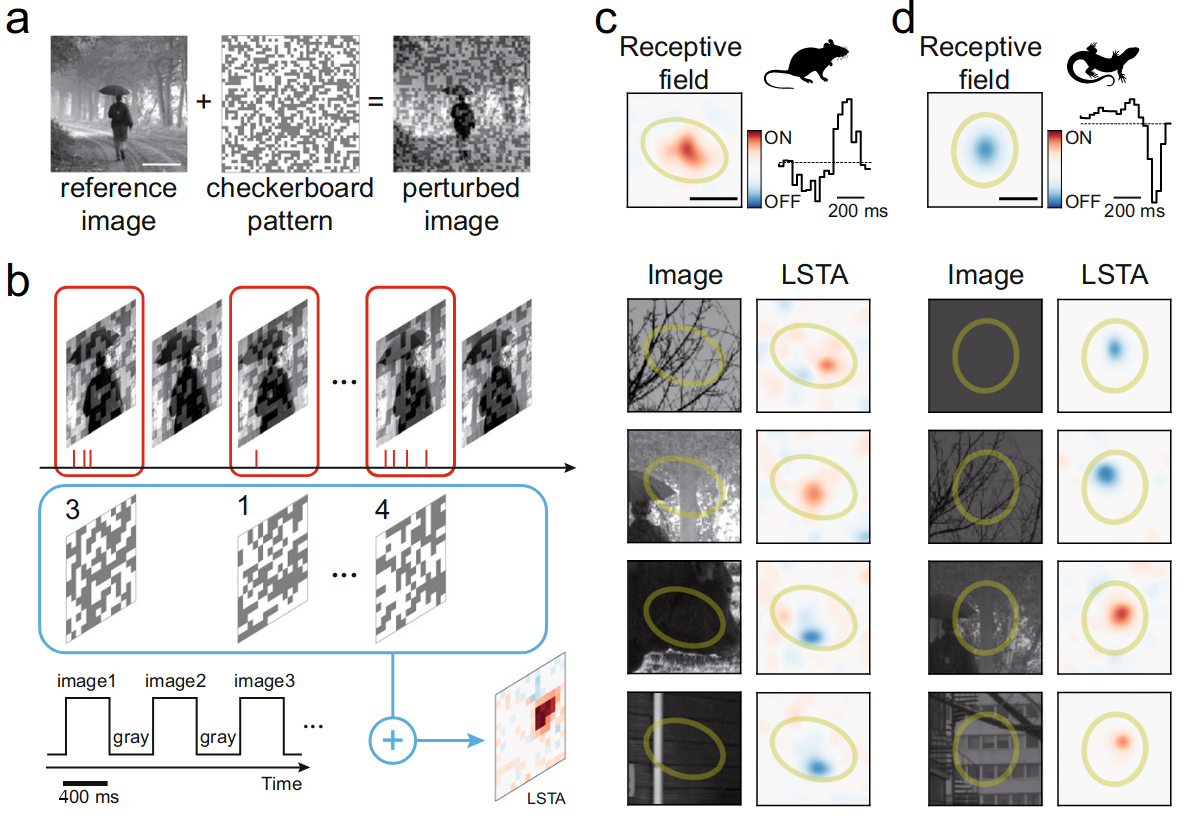
\includegraphics[width=\textwidth]{pics/LSTAExplainV2.png}
    \caption{\textbf{LSTA.}\textit{Adapted from Goldin et al., 2022.} a.
        Natural images are
        perturbed with checkerboards. Scale bar = 500 μm. b. A random sequence
        of
        perturbed natural
        images is being flashed. A gray frame separates all flashes. To compute
        LSTA, we average all different
        perturbations weighed by the number of spikes they evoked. c An example
        of
        LSTA for a cell of the
        retina of a mouse. On top, the spatial and temporal receptive field of
        the
        cell, as is classically used. On
        the bottom, the LSTA of the cell (right) for different natural images
        (left). A green ellipse fitted on
        the classical spatial field is shown on the LSTA for reference. d Same
        as
        c for an axolotl. }
    \label{fig:LSTA}
\end{figure}
% Give details about how the images are built for the camera.

The training set is composed of 3180 clips, each composed of a grey
adaptation image followed by a natural image. The test set is composed of 30
clips, each repeated 30 times, for a total of 900 clips.
The test clips are composed of 10 different natural
images preceded by each adaptation (3 different clips for each natural image).
The dataset used to record LSTA is composed of 9 different clips repeated 1000
times. Each clip is composed of one of the three selected natural images
preceded by one of the adaptation patterns.

We first used 4 different natural images while computing the LSTA of each cell,
each 12 different clips being repeated 12 times. We found that the estimation
of the LSTA was too unstable with only 750 repetitions. In the following
experiments, we excluded the image that yielded the least amount of stable
estimations of LSTA (20\% average success rate as compared to 42\% average
success rate for the other three images). We then used 3 different natural
images while computing the LSTA of each cell, each 9 different clips being
repeated 1000 times. We found that the estimation of the LSTA was more stable
with 1000 repetitions.

\textbf{Data processing.}
Multi-electrode array experimental data takes the shape of a collection of
temporal electrical signals tiling the recorded area.
In most scenarios, including here, these signals are sorted into different cell
signals using a semi-automatic clustering algorithm. This algorithm is based on
the shape
of the electrical spikes as well as their spatial location. It is
quite messy due to the low signal-to-noise ratio in the data and each
experiment needs to have its sorting corrected by hand.
This process can take up to an
entire day for a single experiment. I used spiking-circus for semi-automatic
spike sorting and the UI phy for handmade corrections \citep{yger_spike_2018}.
It is important to note that even though the retina is an easier organ than
most to record clean spike signals from, the data is still very noisy and the
sorting process is not perfect. Hence, when validating hypotheses, cells are
usually rated by their reliability.

% Checkeckerboards and RF
After spike sorting, we analyze the recording from standard stimuli to
characterize each
ganglion cell receptive field. To this end, we display a random binary
checkerboard for approximately 1 h at 30 Hz. Check size is 42\textmu m. A
ganglion cell receptive is computed as its spike trigger average (STA), for
this checkerboard stimulus. The STA of a cell can also be described as the
stimulus that triggers the most spikes from that cell. It is computed as the
average of the presented checkerboard weighted by the number of spikes using a
set number of samples per repetition (here 21). The spatial STA is usually
shown as the 2-dimensional spatial slice at the maximum value after smoothing.
The temporal STA is the one-dimensional time slice at the pixel with the
maximum
value. For smoothing, a double Gaussian is fitted on the resulting spatial
STA.

% Add a figure with a clear viz of STA and RF
% Cell typing (probably useless here, but say a word about it)

\textbf{LSTA.}
To record the local specificity of the response of a ganglion cell to a natural
image, we used a method called local spike trigger average (LSTA) for its
analogy with the STA. This method was previously developed in the laboratory.
We first generate a set of perturbed natural images by superimposing some of
the natural images (3-4 images) with various perturbation patterns in the form
of random checkerboards (Figure \ref{fig:LSTA}). We once again used a checker
size of 42\textmu m.
Following calibration guidelines measures in previous experiments, the
amplitude of the perturbation was set to 12.5\%, where 100\% corresponds to a
pixel value of 1. In the mouse retina, this amplitude was found to trigger a
change in firing rate of approximately 1.5Hz in ganglion cells with high firing
rates to the unperturbed images \citep{goldin_context-dependent_2022}. To avoid
any adaptation to a single reference natural image, we shuffled randomly all
the clips.

As for the STA, the LSTA is computed as the average of the perturbation
patterns weighted by the response of the RGC. The responses are computed by
counting the number of spikes on a time window ranging between +50ms and +450ms
after the display of the natural image. It was chosen to minimize the impact in
the response of delayed spikes due to the perturbation patterns while
maximizing
the capture of spikes that are responses to the natural image.

% FROM NOW ON THERE IS S LOT TO WRITE...
\textbf{Data visualization.}
Due to the complexity of the recorded information, it can be challenging to
have
all the relevant information on one screen. First, it's important to always
have the raster plot in sight since it informs of the quality of the cell at a
glance (Figure \ref{fig:cell_selection}).
Then, we usually display the STA and the LSTA of the cell, typically zoomed on
the cell receptive field (Figure \ref{fig:CellExample}).
Finally, we display the temporal profile of the cell response as the
Poststimulus time histograms
(PSTH). They are histograms of the times at which neurons fire.

% IS THIS PART VAUABLE......

% Add a figure that sums up all the visualization, like a cell summary but with absolutely everything !!!

\textbf{Cell selection.}
Not all recorded cells are suitable for all types of analysis. Overall, the
main quality we look for in a cell is its stability during an entire stimulus
clip.
It reflects its health and likeliness to behave normally during the
presentation. For our most complex experimentations, cells need to remain
stable in vitro for up to five hours, which is quite unlikely. In Figure
\ref{fig:cell_selection}, we
describe the different selection steps. Among the 264 cells
in our last experiment, only 14 passed all of them. Note that a cell doesn't
have to
pass all the tests to be considered for a given analysis. For example, any cell
that passed the 'CNN-Train' could be used to fine-tune the CNN model.
% Graph idea : All types of rasters for one cell

% I got a bit original on that figure, I don't think it's that great but well
\begin{figure}
    \centering
    \vspace*{-3cm}
    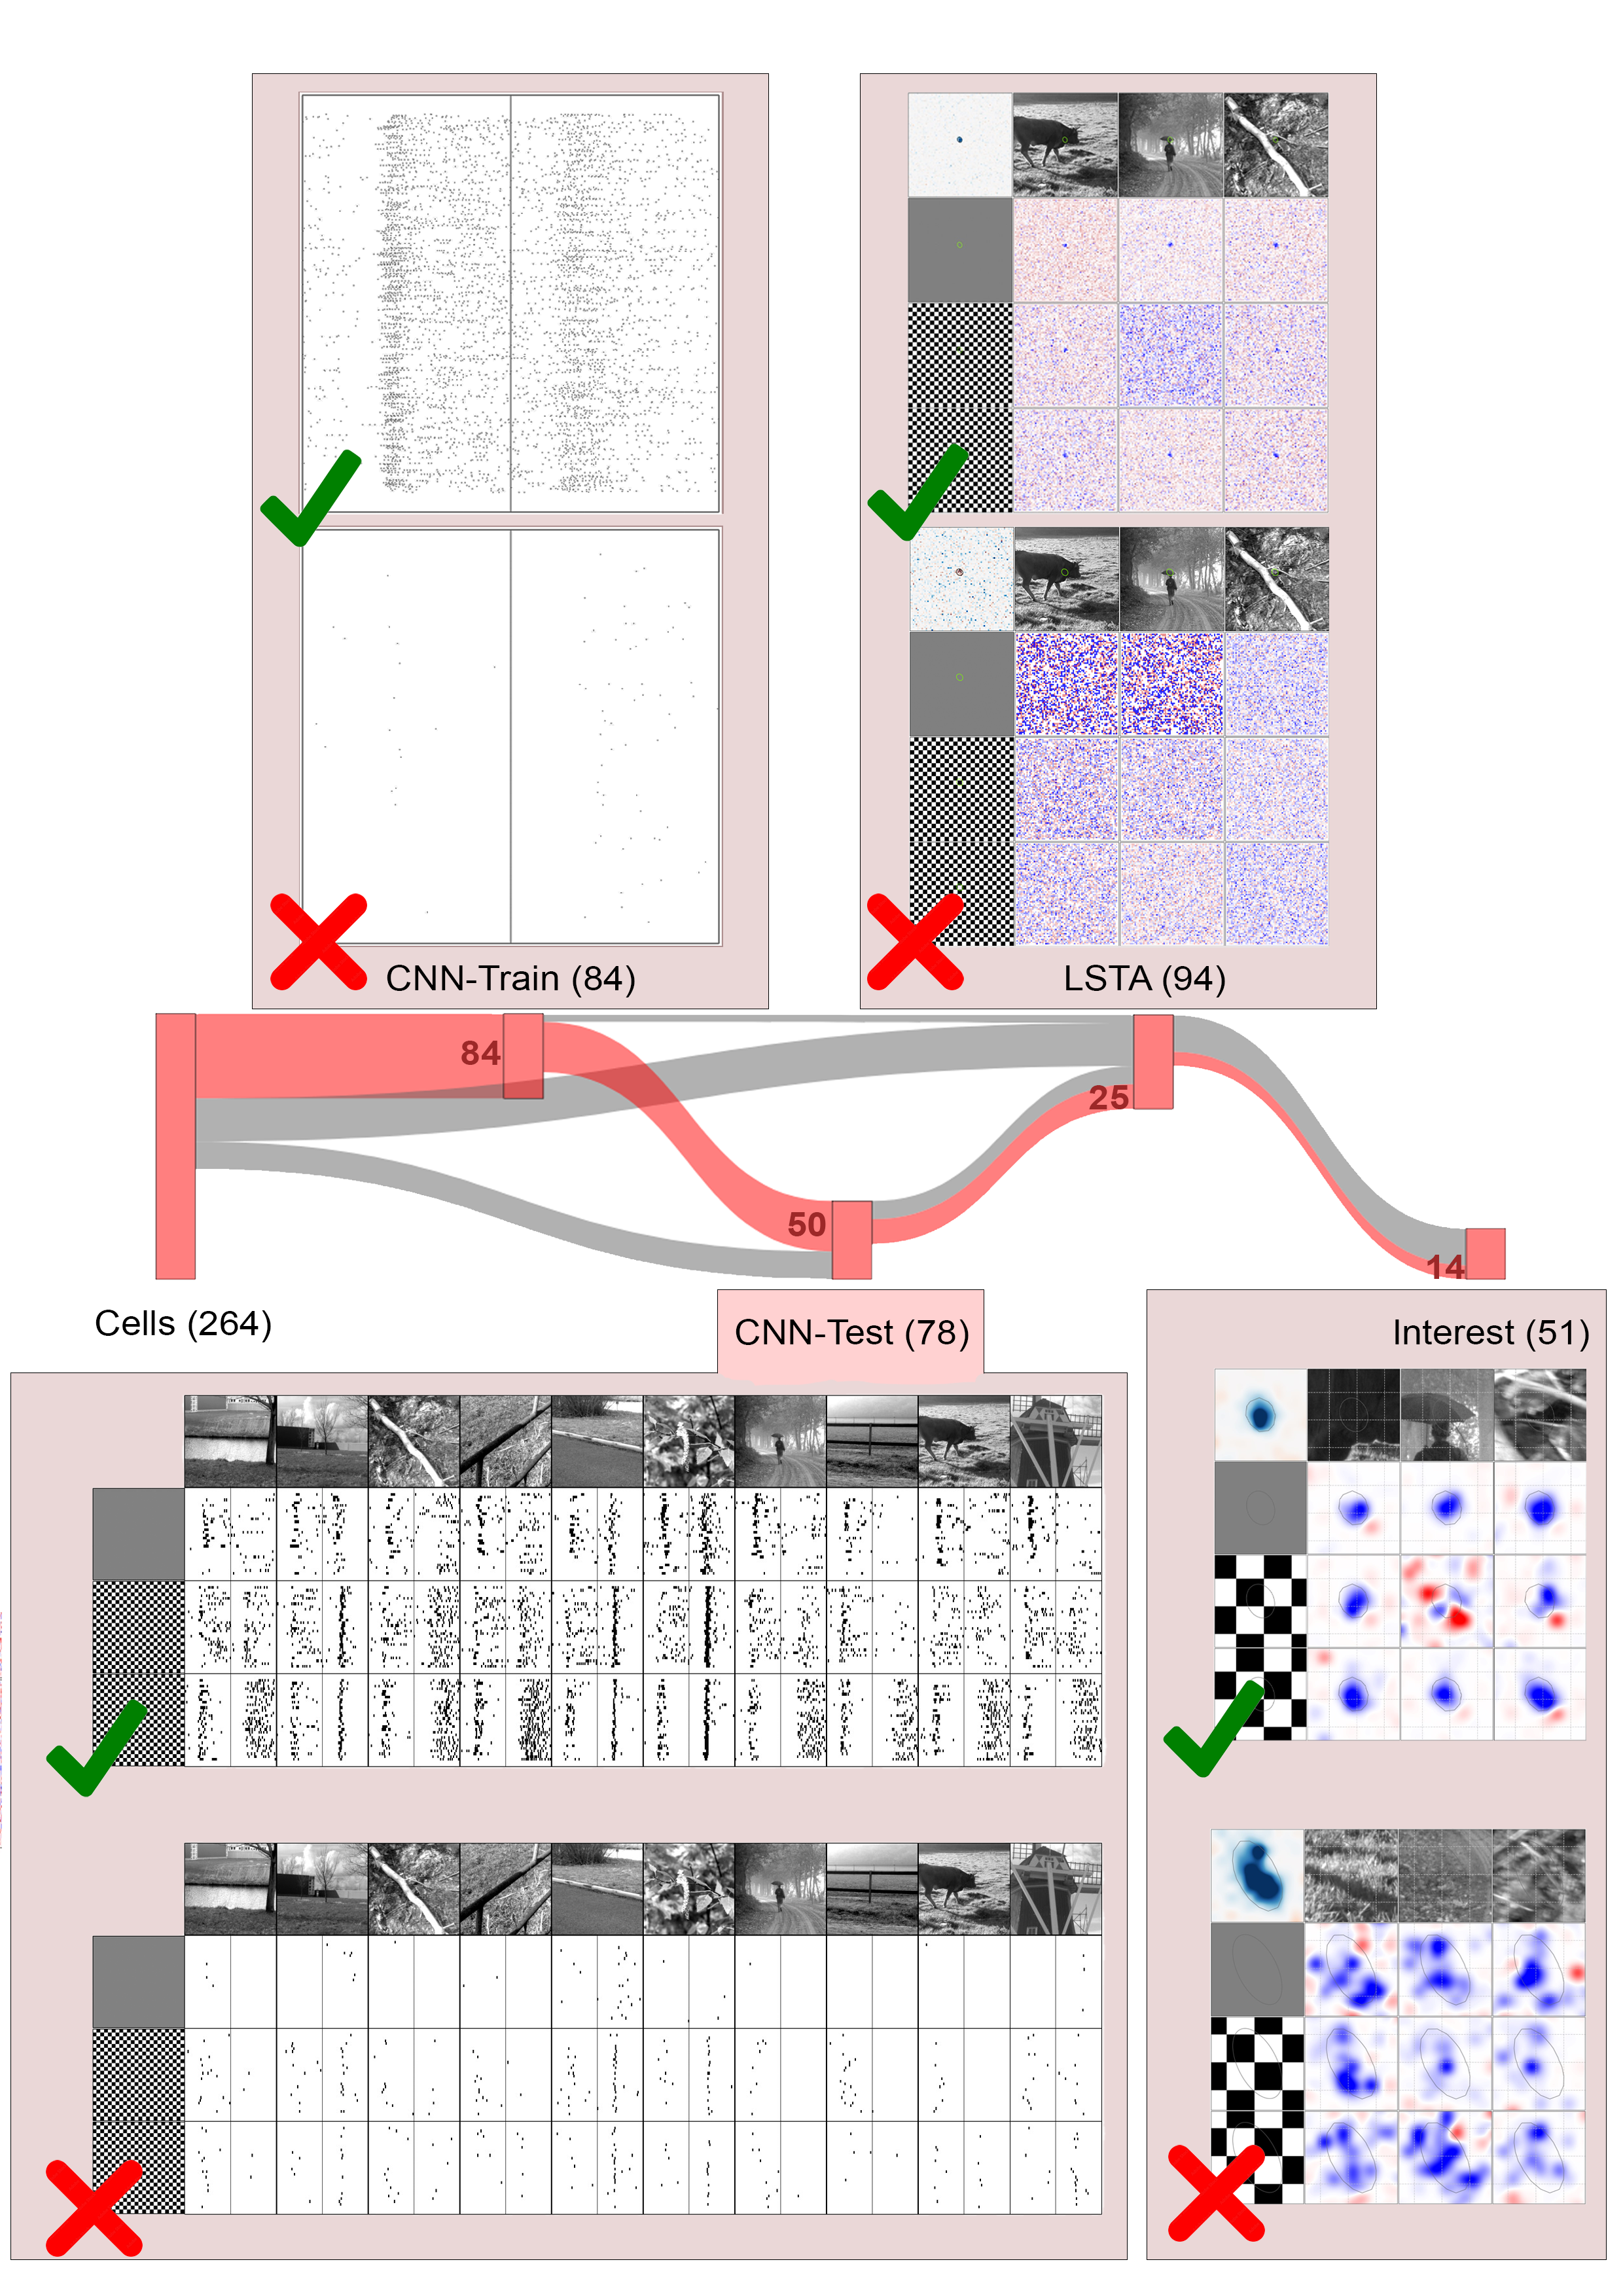
\includegraphics[width=0.8\textwidth]{pics/CellSelection.png}
    \caption{\textbf{Selecting cells suitable for the different degrees
            of
            analysis.} \textbf{Middle.} Flow chart of the cell selection. In
        red, we painted the amount of cells that successively passed each test.
        \textbf{Outer.} Examples of good and
        bad cells
        for each test. On each raster plot, a vertical bar represents the
        instant the natural image was shown, following the adaptation pattern.
        For the
        training dataset, we looked for cells that
        consistently spike on natural images. The more constant the delay, the
        more
        stable the cell. For the test dataset, we looked for cells that gave a
        stable
        response to most of the repeated test clips. For the LSTA analysis, we
        looked
        for cells that showed bright spots in the unfiltered data, to avoid
        confusing
        noise for a signal after smoothing. To determine if the cell had a
        modeling
        interest, we smoothed the LSTA and zoomed on the cell receptive field.
        A cell
        is considered interesting if its LSTA is well-defined for numerous
        pairs. The
        most interesting cells are those where the LSTA is impacted by the
        adaptation
        image.}
    % That description is not clear enough if the rasters are not described somewhere else
    \label{fig:cell_selection}
\end{figure}

% Models: Put the emphasis on the balance between G.C. and data-driven models
% Also insist on the time component of the models

\textbf{Modeling.} This is the most consistent part of my work in the
laboratory, as well as the
most challenging. We are designing a dynamic model of the retinal fast
adaptation.
By comparing how different modeling strategies reproduce the
observed LSTA in the data, we can gain insight into how fast adaptation to
natural scenes is implemented in the retina.
%I think what is missing here is what question you want to answer with this. We should discuss this more. 

We first created a toy model (data-agnostic) of the retina, based on the LNLN
model described
in \ref{sec:background}. By adding a gain control mechanism to the model, we
were able to reproduce some behavior of the LSTA as observed in the data
(Appendix \ref{chap:toyModel}).
This approach is very limited since the numerous non-linearities in the LNLN
the model makes its dynamics very complex.
As an answer, we are fitting a more complex model, based on a convolutional
neural network (CNN), that will be able to infer the non-linearities from the
data. For this report, we'll focus on this part of the modeling since it is
what I've been working on the most.
We are using a deepnet framework, optimized using the
Pytorch library. In practice, we use a model that differs slightly from the
LNLN
model. In Figure \ref{fig:CNN_simple}, we show a simplified view of our
architecture focusing on how the model predicts spikes from a video clip.

Additionally, we are using a few regularization strategies to improve the model
performance as well as ensure it learns filters that are comparable to the
retina. % CHANGE THAT
The subunit filters are regularized using a smoothing constraint, the L2
regularization. The RGC receptive field is regularized using a sparsity
constraint, the L1 regularization, as well as L1. Using a process called batch
normalization, we also ensure that the activation maps as well as the feature
scores matrix stay around 0 while not taking too small values that would
produce numerical errors. Finally, to partially avoid overfitting on the
training set, we added a dropout layer between the subunits and the RGC
receptive field.

Each trial of the model was optimized using the Adam optimizer, with varying
learning rates. The loss function is the Negative log-likelihood loss with
Poisson distribution of target. It is a standard loss function for predicting
rare events such as neural spikes.
The hyperparameters of the regularizations were optimized using a random grid
search strategy, using a pipeline recently developed within the laboratory.
% ADD REFERENCE

All the code was written in Python and is mainly built around the Pytorch
library \citep{pytorch}.
We thought the explanations of those concepts were out of the scope of the main
text of this report. A more accurate and mathematical description of the model,
the regularizations and the optimization strategy can be found in the Appendix
\ref{app:CNN}.

As an indication, one trial of the model takes approximately 2 hours to train.
The current results of this project are already the results of more than one
month of consecutive computation.

\begin{figure}
    \centering
    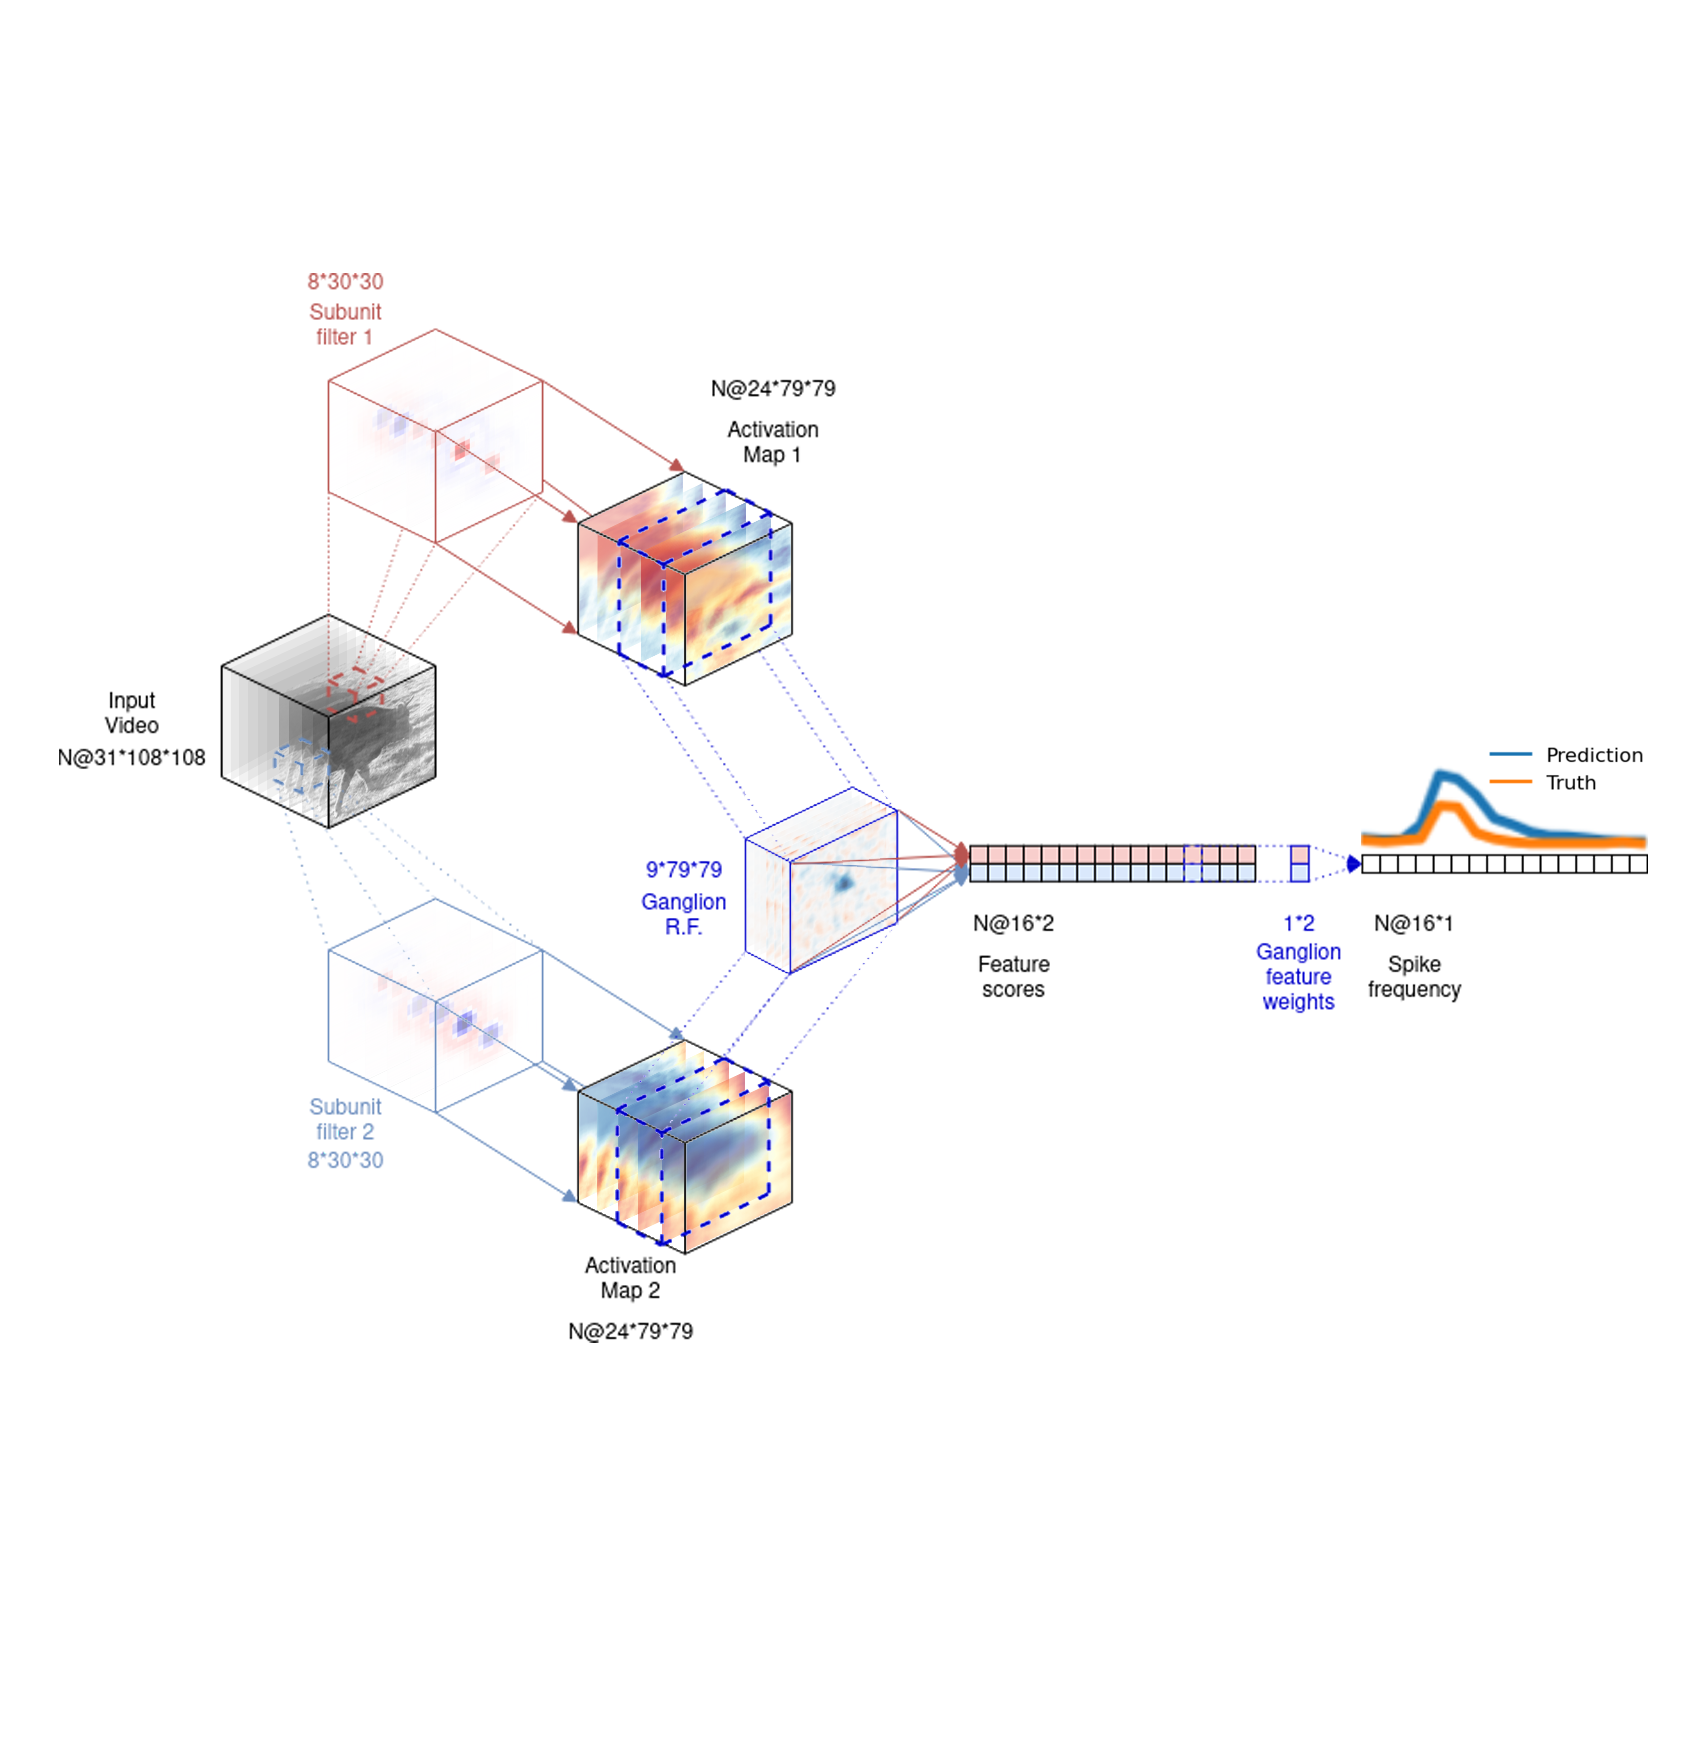
\includegraphics[width=\textwidth]{pics/CNNSimpleWithImgs.png}
    \caption{\textbf{From stimulus to prediction in the CNN model.} Elements in
        black are the input and consecutive outputs while colored
        elements
        represent the model layers. Lines with arrows represent a convolution
        (the
        filter is dragged upon the input to produce the output, usually of
        smaller
        dimensions), while pointed lines represent a zoom on a given layer. N
        is the size of the batch. The subunit filters and the ganglion feature
        weights layer end
        with a non-linearity (ReLU and SoftPlus respectively).
        Each subunit filter (here only two are shown) represents the
        selectivity
        of a subunit (one can think of them as bipolar cells). Each subunit
        type covers the entire input spatially. They also integrate temporal
        events on a given number of frames. Each pixel of the
        activation maps encodes the level of activation of that subunit in that
        particular location and at that particular instant.
        The RGC receptive field is similar instead that it tiles the entire
        spatial input. It could be described as a pooling of the subunit
        activation
        maps. The RGC is modeled to also integrate temporal events on a given
        number of frames. This spatiotemporal receptive field is the same for
        all
        subunits but the scores corresponding to each subunit pathway are
        different.
        Finally, the feature weights represent how much of each feature is
        relevant foe
        determining the spiking frequency on a given temporal bin. This layer
        is just
        a weighted average of the two features and a non-linearity.
    }
    \label{fig:CNN_simple}
\end{figure}

\textbf{Model evaluation.}
To evaluate the performance of the models, we used a testing set of 30
different stimuli where each stimulus has been repeated 30 times as described
in \textbf{Stimulus design}.
We computed single-trial correlations $\rho$ between the ground truth and the
prediction following the following steps:
\begin{enumerate}
    \item We defined the ground truth as the average firing rate over all
          repetitions of the same stimulus.
    \item We standardized both the ground truth and the prediction by
          subtracting the mean and dividing by the standard deviation of each group
          respectively. This is to take into account that the output of the model is not
          necessarily on the same scale as the ground truth.
    \item We computed the Pearson correlation between the two vectors.
\end{enumerate}
% I can add this if I have time to actually do it before Sunday

\clearpage